%author: Dorian VOLPE
\subsubsection{HTLC}

Un HTLC est un type de \textit{smart contract} utilisé dans les applications \textit{blockchain} qui réduit le risque de contrepartie en créant une garantie basée sur le temps et une autre sur un verrou cryptographique.
Ils reposent sur deux primitives fondamentales: le verrou de hachage et le verrou temporel.\\
Premièrement le verrou de hachage (ou bien \textit{hashlock}): Ce dernier va fonctionner comme une assurance qui va couvrir les parties participantes à la transaction, en leur garantissant que chaque modification de l'échange soit réalisée d'un commun accord de toutes les parties.
Cela est mis en place grâce à un partage du hachage de la clef privée de la transaction, ce partage va donc impliquer que le canal de paiement mis en place ne puisse être ouvert ou fermé qu'avec l'accord de tous les participants.\\
Ensuite le verrou temporel (ou bien \textit{timelock}) va laisser un laps de temps prédéterminé afin que chaque côté du canal puisse prendre ses dispositions avant d'effectuer la transaction. Si jamais ce temps est écoulé alors la clause secondaire du contract (elle aussi prédéterminée) sera exécuté. 
Dans la plupart des cas cette clause secondaire va simplement fermer le canal de paiement et terminer la transaction sans la diffuser sur une \textit{blockchain}.\\
L’intérêt principal de ce type de contrat est qu'il permet d'effectuer facilement des échanges hors chaines. En effet, vu que les participants s'accordent au préalable sur le montant de la transaction ils peuvent tout à fait réaliser l'échange sur des \textit{blockchains} différentes, sous réserve que ces \textit{blockchains} aient des mécanismes de \textit{smarts contracts}.

\begin{figure}[h!]
    \centering
    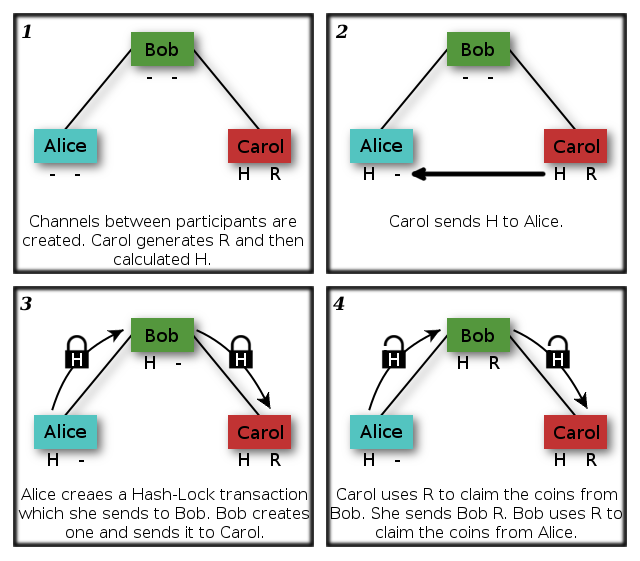
\includegraphics[scale=0.35]{decentralisation/Timed-HashLocks-Diagram-Image.png}
    \caption{Utilisation basique d'un HTLC}
    \label{fig:HTLC}
\end{figure}
\subsubsection{Atomic swaps}
Les \textit{atomics swaps} ou bien échanges atomiques sont des échanges effectués entre deux \textit{blockchains}. On les appelle "atomiques" car il respecte une primitive essentielle à leur fonctionnement et à leur principe d'utilisation: 
l'échange est insécable, c'est-à-dire qu'a son issue, soit il s'est pleinement exécuté, soit l'état antérieur à l'échange est préservé.
Cette primitive permet de garantir que les participants ne seront jamais dans des états jugés "inacceptables". \\
En effet les échanges atomiques partent du postulat que si une partie suit le protocole à la lettre alors, 
il ne sera jamais perdant. A contrario les partis ne suivant pas le protocole par malveillance ou par erreur, prennent le risque de perdre leurs mises de départ.\\ \\
Lors d'un échange atomique les HTLC vont être utilisés de manière centrale car ils vont permettre d'apporter les garanties que nous avons vue dans la partie précédente. Il faut voir les échanges atomiques comme une généralisation de l'utilisation des HTLC. Lors d'un échange atomique les deux \textit{blockchains} mises en relation doivent pouvoir communiquer et échanger sur une interface commune comme un portefeuille multi signature ou un canal d'échange mis en place spécialement pour cette transaction. \\ \\
Si nous nous penchons sur le déroulement d'un échange atomique à deux parties nous pouvons déduire les étapes suivantes: 
\begin{enumerate}
    \item Les deux parties participent à l'échange, créant un HTLC (sur chaque \textit{blockchain}) dans lequel les fonds sont bloqués. 
    \item Les deux parties échangent les informations nécessaires pour effectuer une transaction sur la \textit{blockchain} de l'autre partie. 
    \item Les deux parties vérifient l'exactitude des informations reçues et signent la transaction. 
    \item Les événements sont envoyés sur les \textit{blockchains} respectives. 
    \item Les transactions sont confirmés par les \textit{blockchains} respectives et les fonds sont débloqués.
\end{enumerate}

\begin{figure}[h!]
    \centering
    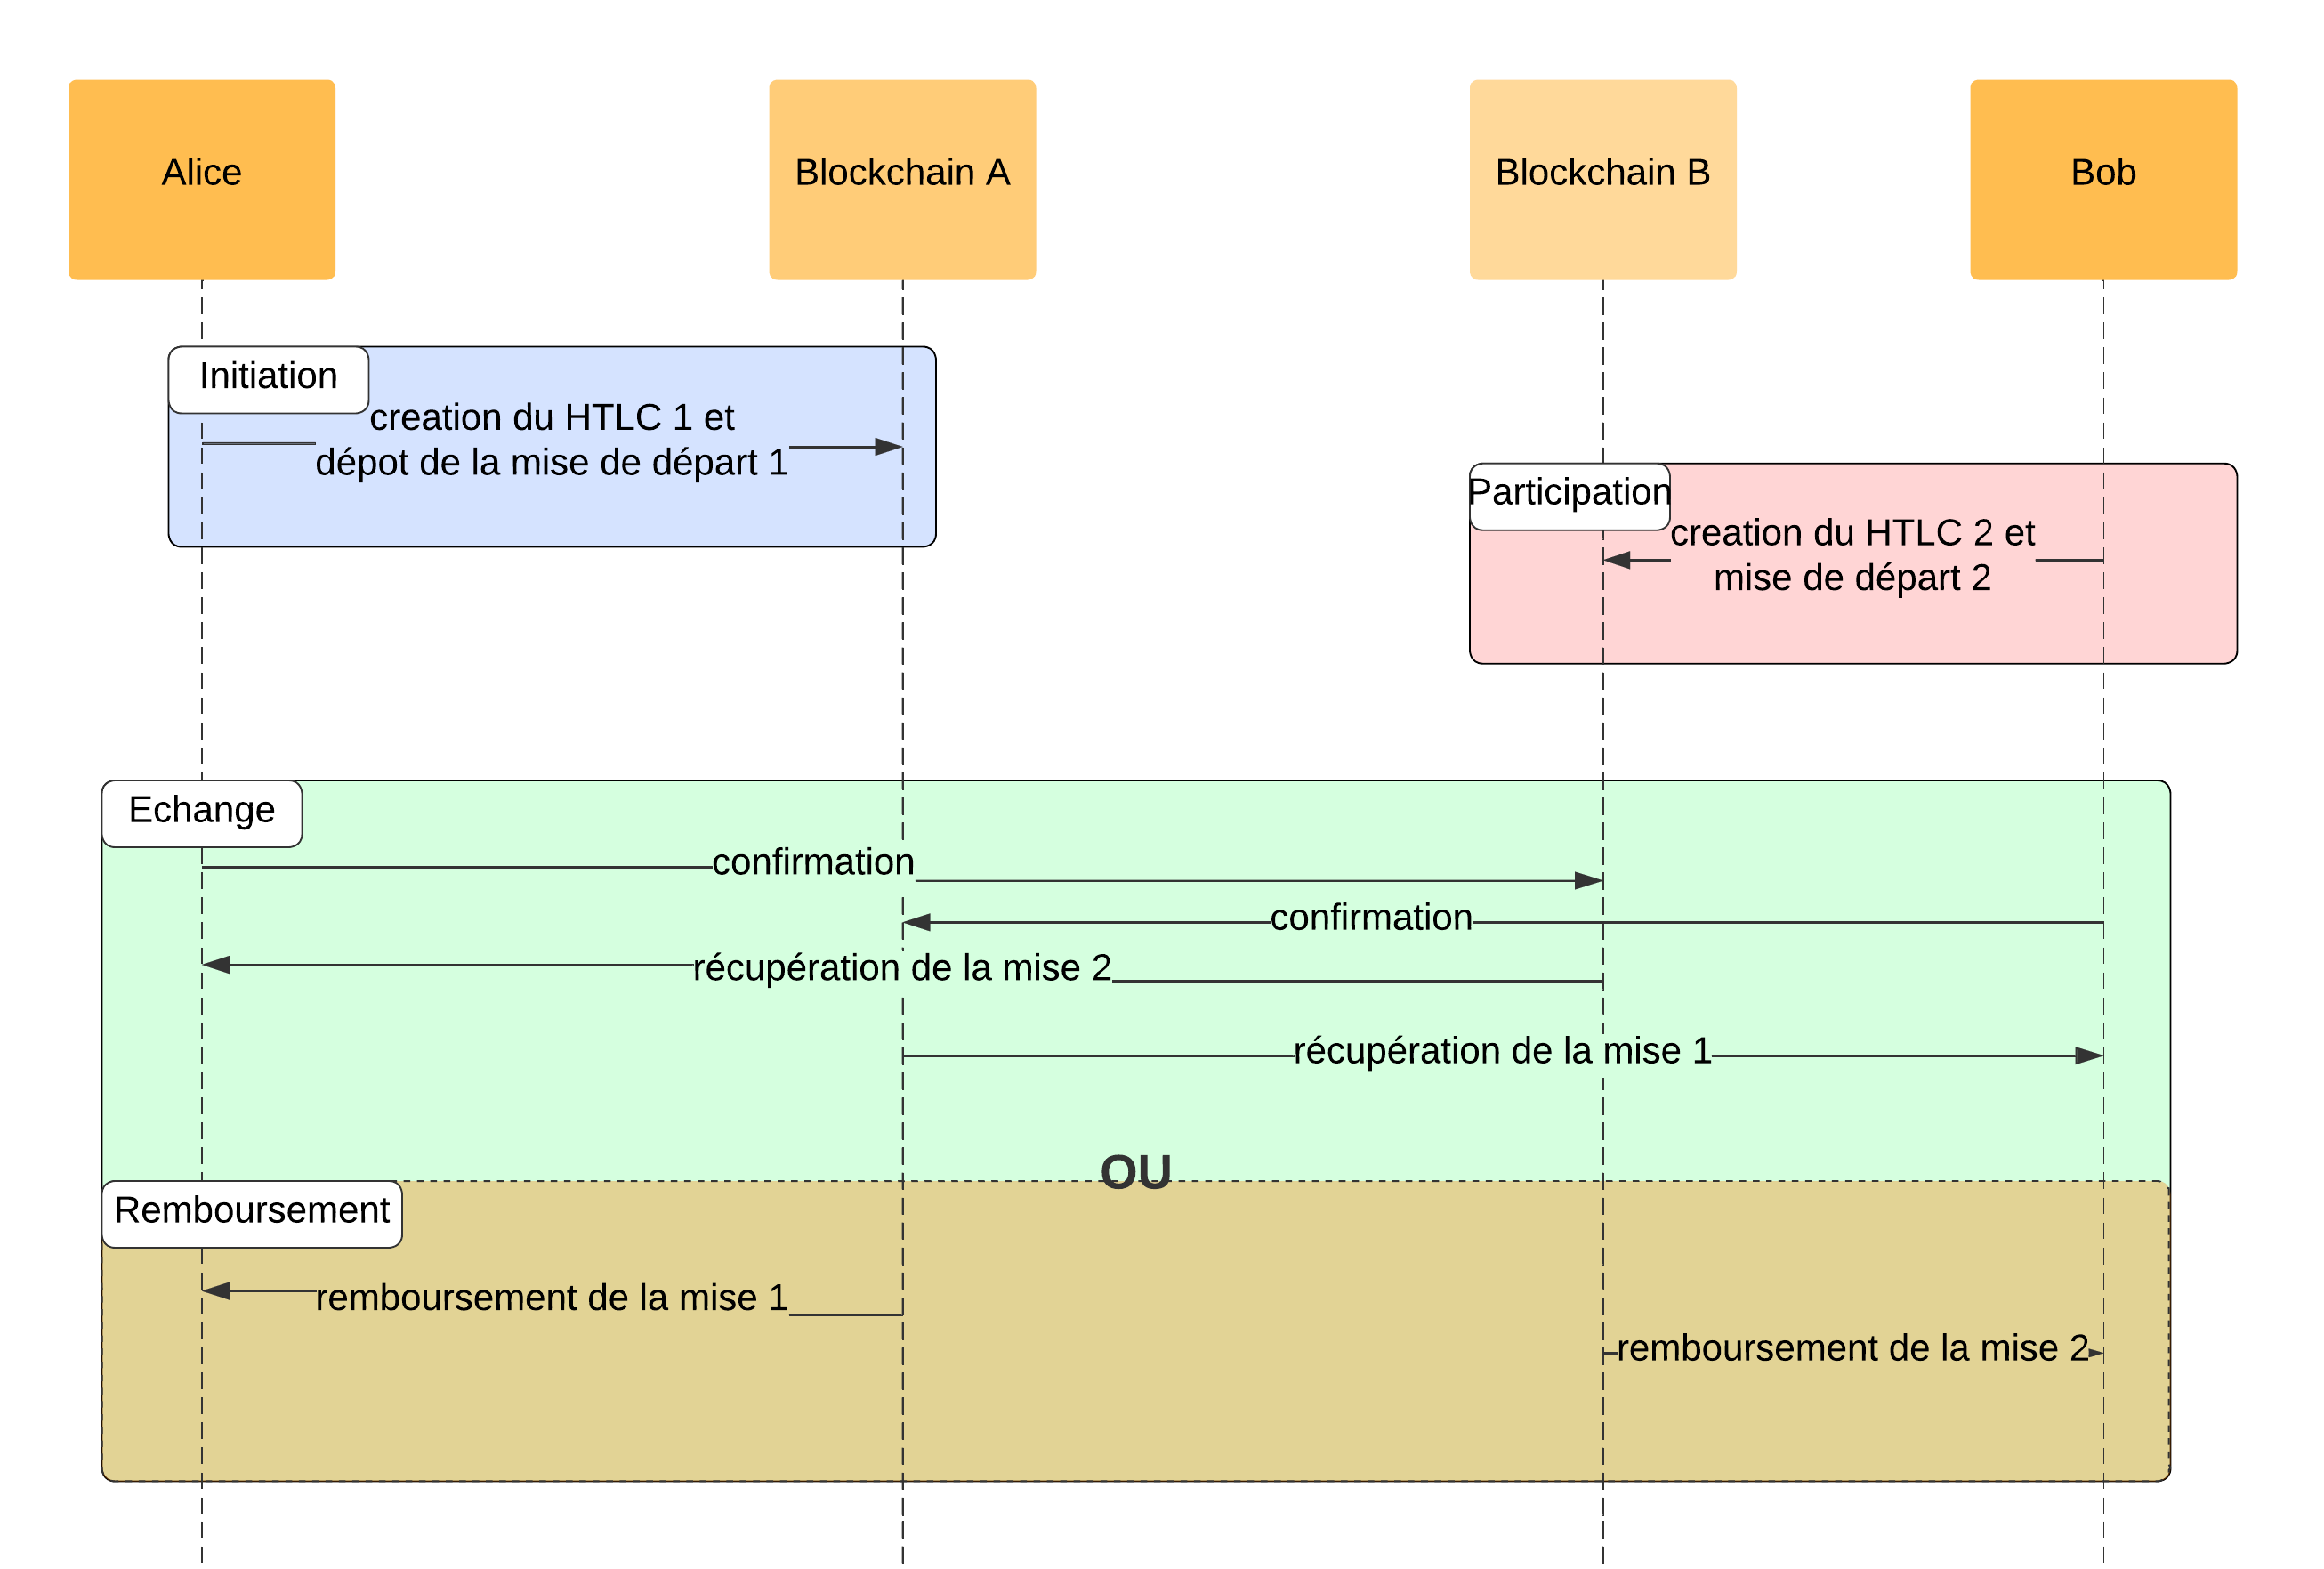
\includegraphics[scale=0.15]{decentralisation/atomicSwap.png}
    \caption{Déroulement simplifié d'un échange atomique}
    \label{fig:atomicSwap}
\end{figure}

